%!TEX root = main.tex
\subsection{From Single to Dueling}
To generalize learning across actions without imposing any change to the underlying reinforcement learning algorithm, Ziyu Wang \textit{et al.}\cite{wang2015dueling} proposed dueling Q-network.

\begin{figure}[ht!]
	\centering
	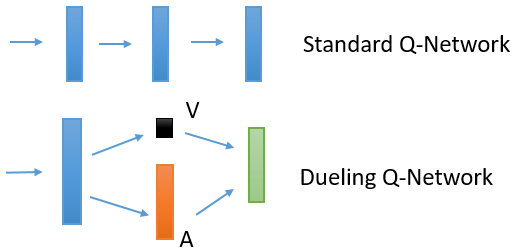
\includegraphics[width=0.49\textwidth]{./fig/dueling.png} \\
	\caption{The architecture of Dueling Q-Network.}
	\label{fig:dueling_q_network}
\end{figure}

As shown in Fig.\ref{fig:dueling_q_network}, The top one is standard Q-network which has only one stream. 
%
The dueling network has two-streams in the middle. One is called $V value$, which denotes how good it is to be in the current state. The other is called $Advantage$, which represents how good is every action.
%
As a result, the dueling Q-network can learn which states are valuable, without having to learn the effect of each action for each state. 

\subsection{Experience Replay}

During sampling, we adopt \textit{experience replay}\cite{adam2012experience} in order to stabilizing the training process.
%
The basic idea is that through keeping an agent’s experiences , we can randomly sample experiences from memory and breaks the time correlation of the data.
%
Specifically, by keeping the experiences, the Q-network can avoid learning about what it is immediately doing in the environment, and it can learn from the past experiences. 
%
These experiences are stored as tuples of \textit{(state,action,reward,next state)} and updated online. (As new experiences come in, old ones are removed randomly). 
%
When optimizing, we simply sample a uniform batch of random experiences from memory, and train our network with them.
%
As shown in Fig.\ref{fig:experience_replay}, we first sample the experiences from environment randomly, which means for every given state $s$, we take a random action $a$ and record the new state $s'$ and new reward $r'$.

\begin{figure}[ht!]
	\centering
	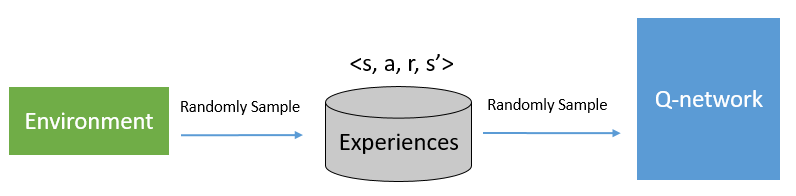
\includegraphics[width=0.49\textwidth]{./fig/experience_replay.png} \\
	\caption{Illustration of experience replay.}
	\label{fig:experience_replay}
\end{figure}

\subsection{Target Network}
To reduce the oscillation during training, we employ Target Network Strategy\cite{lillicrap2015continuous}.
%
Specifically, at every step of training, the target Q-values are shifting if we use the same network to produce target Q-values.
%
If we are using a constantly shifting target Q-values to optimize our Q-network, the updates can easily run out of control and fall in local optima. The estimates of Q-values will then be inaccurate.
%
The idea behind target network is that it utilizes a second network called target network which has exactly the same architecture as original one during the training procedure.
%
The target network is used to generate the target Q values. The target Q-values are used to compute the loss during training.
%
In order to mitigate that risk, the target network’s weights are fixed for a number of iterations, and periodically or updated to the original Q-networks values. 
%
we can achieve more stable training procedure if target network strategy is used.

\subsection{Experiment Results}


In this experiment, we investigate the benefits of using \textit{experience replay} and \textit{target Q-network}
%
As we can see in Fig.\ref{fig:target_network_result}, using target Q-network can reduce the oscillation during training and increase the converge speed.
%
In Fig.\ref{fig:er_result}, we can see that even though using experience replay costs us 400 steps for accumulation, the network quickly converges after that. And the oscillation is very small.
%
These two experiments show that using \textit{Experience replay} and \textit{Target Q-network} can improve the training process.


\begin{figure}[ht!]
	\centering
	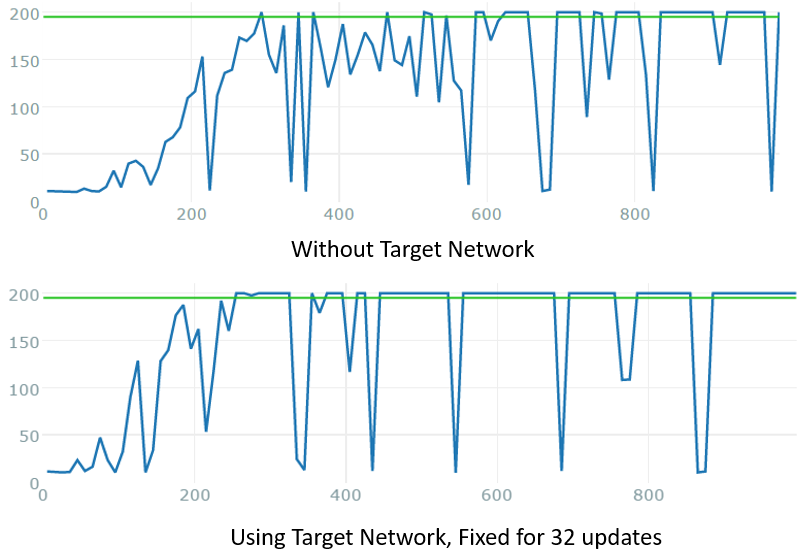
\includegraphics[width=0.49\textwidth]{./fig/target_network_result.png} \\
	\caption{Benefit of using target Q-network.}
	\label{fig:target_network_result}
\end{figure}

\begin{figure}[ht!]
	\centering
	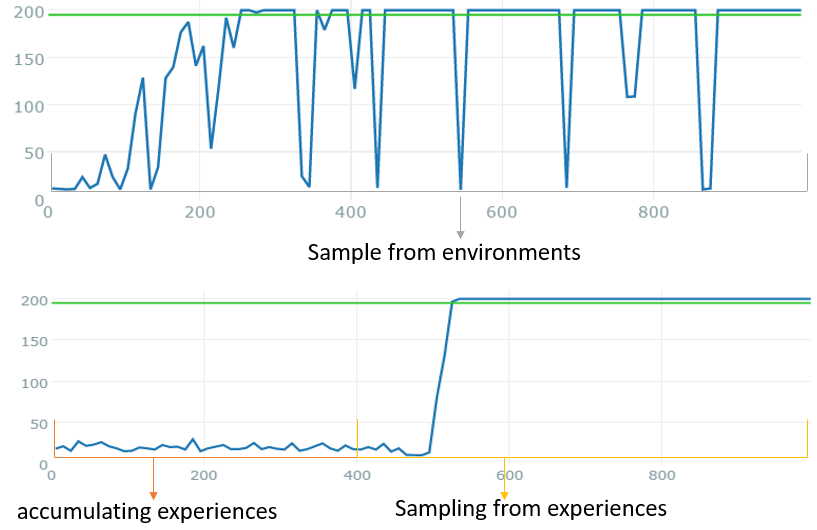
\includegraphics[width=0.49\textwidth]{./fig/er_result.png} \\
	\caption{Benefit of using experience replay.}
	\label{fig:er_result}
\end{figure}


